\documentclass{beamer}
\setbeamercovered{transparent}
\setbeamertemplate{footline}[frame number]
\setbeamertemplate{navigation symbols}{}
\usetheme{Montpellier}
\usecolortheme{crane}
\usecolortheme{rose}
\usecolortheme{seahorse}

% Packages
\usepackage{graphicx} % For diagrams
\usepackage{stmaryrd} % For integer interval
\usepackage{algorithm, algpseudocodex} % For natural code
\usepackage{hyperref} % For hyperlinks

\usepackage{color}
\usepackage{listings} % For code inlusion
\usepackage{multicol} % For annexe
\usepackage{tabularx} % For tables
%

% Make summary
\AtBeginSubsection[]
{
    \begin{frame}
        \frametitle{Plan}
        \tableofcontents[currentsection, currentsubsection]
    \end{frame}
}

\AtBeginSection[]
{
    \begin{frame}
        \frametitle{Plan}
        \tableofcontents[currentsection]
    \end{frame}
}
%

% Rename keywords
\renewcommand{\algorithmicrequire}{\textbf{Entrée:}}
\renewcommand{\algorithmicensure}{\textbf{Sortie:}}
% \renewcommand{\algorithmiccomment}[1]{\{#1\}}
\renewcommand{\algorithmicend}{\textbf{fin}}
\renewcommand{\algorithmicif}{\textbf{si}}
\renewcommand{\algorithmicthen}{\textbf{alors}}
\renewcommand{\algorithmicelse}{\textbf{sinon}}
\renewcommand{\algorithmicfor}{\textbf{pour}}
\renewcommand{\algorithmicforall}{\textbf{pour tout}}
\renewcommand{\algorithmicdo}{\textbf{faire}}
\renewcommand{\algorithmicwhile}{\textbf{tant que}}
\renewcommand{\algorithmicreturn}{\textbf{renvoyer}}
\renewcommand{\algorithmicprocedure}{\textbf{procédure}}
\newcommand{\algorithmicelsif}{\algorithmicelse\ \algorithmicif}
\newcommand{\algorithmicendif}{\algorithmicend\ \algorithmicif}
\newcommand{\algorithmicendfor}{\algorithmicend\ \algorithmicfor}
\floatname{algorithm}{Algorithme}
%

% Custom commands for animating frames
\newcommand{\animframe}[1]{
    \addtocounter{framenumber}{-1}
    \begin{frame}
        \noindent
        \begingroup
        \centering
        \makebox[0pt]{\includegraphics[width=12cm]{#1}}\par
        \endgroup
    \end{frame}
}
%

\title{Peut-on factoriser suffisamment rapidement les nombres en facteurs premiers?}
\author{Tristan Delcourt, Louise Nguyen}
\date{2025}

\begin{document}

\begin{frame}[plain]
    \titlepage
\end{frame}

\section{Introduction et enjeux}
\begin{frame}{Les nombres \textit{RSA}}

\begin{itemize}
    \item Factoriser $N = pq$ où $p$ et $q$ sont premiers et très grands.
    \item Dernier nombre non factorisé: RSA-260 (260 chiffres)
        \newline
        \newline
        $N=221128255295296664352810852550262309276120895\allowbreak
        0247001539441374831912882294140200198651272972656\allowbreak
        9746599085900330031400051170742204560859276357953\allowbreak
        7571859542988389587092292384910067030341246205457\allowbreak
        8456641366454068421436129301769402084639106587591\allowbreak
        4794251435144458199$
\end{itemize}

\end{frame}

\section{La méthode de Dixon}
\subsection{Congruences de carrés}
\begin{frame}{Congruence de carrés}

\uncover<+->{$N = pq$, $p$ premier. Supp. $x^2 \equiv y^2 \pmod N$ et $x\neq\pm y$.}
\begin{itemize}[<+->]
\item On a $x^2 - y^2 \equiv 0 \pmod N$ i.e. $N \mid (x-y)(x+y)$
\item Donc $p \mid (x-y)(x+y)$
\item Lemme d'Euclide: par exemple $p \mid x-y$
\item Alors $p$ divise $N$ et $x-y$: $p \mid N \land (x-y)$, ce qui donne $\mathbf{N \land(x-y)\neq1}$
\end{itemize}

\uncover<+->{\begin{block}{Conclusion}
$N \land(x-y)$ et $N \land (x+y)$ sont des facteurs non-triviaux de $N$
\end{block}}
    
\end{frame}

\subsection{Etapes de la méthode}

{
\setbeamertemplate{headline}{}
\setbeamertemplate{navigation symbols}{}

\animframe{diagrams/anim_construction_x_y/part1.png}
\animframe{diagrams/anim_construction_x_y/part2.png}
\animframe{diagrams/anim_construction_x_y/part3.png}
\animframe{diagrams/anim_construction_x_y/part4.png}
\animframe{diagrams/anim_construction_x_y/part4(bis).png}
\animframe{diagrams/anim_construction_x_y/part5.png}
\animframe{diagrams/anim_construction_x_y/part6.png}
}

\begin{frame}{Construction de $y$ - Pivot de Gauss}
    \begin{itemize}[<+->]
        \item On a $b+1$ vecteurs de $\mathbb F_2^b$ et $\mathbb F_2$ corps, cela donne un système lié:
        $$
        \exists (\lambda_i)_{i \in \llbracket 1,b+1 \rrbracket}\in \mathbb \{0,1\}^{b+1} \mid \sum_{i=1}^{b+1} \lambda_iv_i = 0_{\mathbb F_2^b} = (2\alpha_1, \dots, 2\alpha_b)
        $$
        On pose $y = \prod_{j=1}^b p_j^{\alpha_j}$ et $x = \prod_{j=1}^{b+1}x_j^{\lambda_j}$ 
        \item On peut trouver les $\lambda_i$ avec un système que l'on résout avec un \textbf{pivot de Gauss}.
    \end{itemize}
    \uncover<+->{\begin{block}{Résultat admis (calcul)}
    $x ^2 \equiv y ^2 \pmod N$
    \end{block}}
\end{frame}


\begin{frame}{Un exemple}
    \begin{itemize}
        \item $N = 20382493 = 3467 \times 5879$ et $b = 4$, $(2, 3, 5, 7)$
        \item Ces $5=b+1$ nombres $x_j$ vérifient $ x_j^2 \pmod N = 2^{v_j^{(1)}}\cdots 7^{v_j^{(4)}}$:
            \begin{center}
                \begin{tabular}{|c|c|}
                    \hline
                    $x_j$ & $v_j$ \\
                    \hline \hline
                    $16853$ & $(6,5,2,2)$\\
                    \hline
                    $32877$ & $(3,0,7,0)$\\
                    \hline
                    $35261$ & $(3,2,1,0)$\\
                    \hline
                    $48834$ & $(0,2,3,1)$\\
                    \hline
                \end{tabular}
            \end{center}
    \end{itemize}
\end{frame}

\begin{frame}

\uncover<+->{    
    \begin{block}{}
    {\footnotesize
        \begin{columns}
            \column{.7\textwidth}
            \begin{itemize}
            \item $N = 20382493 =$ \alert<6>{$3467$} $\times$ \alert<6>{$5879$} et $b = 4$.
            \item $x_j^2 \pmod N = 2^{v_j^{(1)}}\cdots 7^{v_j^{(4)}}$ pour $j = 1,2,3,4,5$ ($5 = b+1$ relations)
            \end{itemize}
            \column{.3\textwidth}
            \begin{tabular}{cc}
                    $x_j$ & $v_j$ \\
                    $16853$ & $(6,5,2,2)$\\
                    $32877$ & $(3,0,7,0)$\\
                    $35261$ & $(3,2,1,0)$\\
                    $48834$ & $(0,2,3,1)$\\
            \end{tabular}
            \end{columns}
    }
    \end{block}
}

{\small
\begin{columns}
\column{.55\textwidth}
\begin{itemize}[<+->]
    \item On résout dans $\mathbb F_2^5$
    \[
    \begin{cases}
    6\lambda_1 + 3\lambda_2 + 5\lambda_3 + 0\lambda_4 + 3\lambda_5 = 0_{\mathbb F_2} \\
    5\lambda_1 + 0\lambda_2 + 3\lambda_3 + 2\lambda_4 + 2\lambda_5 = 0_{\mathbb F_2} \\
    2\lambda_1 + 7\lambda_2 + 0\lambda_3 + 3\lambda_4 + 1\lambda_5 = 0_{\mathbb F_2} \\
    2\lambda_1 + 0\lambda_2 + 1\lambda_3 + 1\lambda_4 + 0\lambda_5 = 0_{\mathbb F_2} \\
    \end{cases}
    \]
    $\lambda = (1, 1, 1, 0, 1)$ solution.
\end{itemize}

\column{.45\textwidth}
\begin{itemize}[<+->]
    \item $x = \prod_{j=1}^{b+1}x_j^{\lambda_j} = 7248176$ \\ $y = \prod_{j=1}^b p_j^{\alpha_j} = 4837786$
    \item On a $x^2 \equiv y^2 \pmod N$
    \item $N \land (x-y) =$ \alert<6>{$5879$} et $N \land  (x+y) =$ \alert<6>{$3467$}.
\end{itemize}

\end{columns}
}
\end{frame}

\begin{frame}{Ce qu'il faut retenir}
    \begingroup
    \setbeamercolor{block title}{bg=pink, fg=black}
    \begin{block}{Le résultat principal}
        Étant donné $b\in \mathbb B$, trouver $b+1$ nombres tels que $\forall j\in\llbracket 1, b+1\rrbracket, x_j^2 \pmod N$ a ses facteurs premiers inferieurs à $p_b$
    \end{block}
    \endgroup
\end{frame}

\subsection{L'algorithme final}

\begin{frame}{L'algorithme final}
    \begin{algorithm}[H]
    \caption{Recherche de nombres B-friables}
    \small
    \begin{algorithmic}[1]
        \Require{$N \in \mathbb N$ composé, $b \in \mathbb N$}
        \Ensure{$(v_i)_{i \in \llbracket 1,b+1 \rrbracket}, (x_i)_{i \in \llbracket 1,b+1 \rrbracket}$}
        \Statex
        \For{$i\gets1 \dots b+1$}
            \State $en\_cours \gets V$
            \While{$en\_cours$}
                \State{$x_i \gets \mathbb U(1, N-1)$}
                \State $x_i' \gets x_i^2 \bmod N$
                \If{$x_i'$ est $B$-friable (par algorithme naïf)}
                    \State $en\_cours \gets F$
                    \State $v_i \gets (v_i^{(1)}, \dots, v_i^{(b)})$
                \EndIf
            \EndWhile
        \EndFor
        \Statex
        \Return $(v_i)_{i \in \llbracket 1,b+1 \rrbracket}, (x_i)_{i \in \llbracket 1,b+1 \rrbracket}$
    \end{algorithmic}
    \end{algorithm}
\end{frame}

\begin{frame}{L'algorithme final}
    \begin{algorithm}[H]
    \caption{Factorisation par la méthode de Dixon}
    \begin{algorithmic}[1]
        \Require{$N \in \mathbb N$ composé, $B \in \mathbb N$}
        \Ensure{$p$ et $q$, tels que $p\mid N$ et $q\mid N$}
        \Statex
        \State $b \gets\pi(B)$
        \State $(v_i)_{i \in \llbracket 1,b+1 \rrbracket}, (x_i)_{i \in \llbracket 1,b+1 \rrbracket} \gets Recherche BFriables(N, b)$
        \State $(\lambda_i)_{i \in \llbracket 1,b+1 \rrbracket} \gets PivotdeGauss((v_i)_{i \in \llbracket 1,b+1 \rrbracket})$
        \State $x \gets \prod_{j=1}^{b+1}x_i^{\lambda_i}$
        \State $y \gets \prod_{j=1}^b p_j^{\alpha_j}$
        \Statex
        \Return $N \land(x-y), N\land(x+y)$
    \end{algorithmic}
    \end{algorithm}
\end{frame}

\begin{frame}{Etude théorique (Louise Nguyen)}
    \begin{block}{Une minoration de la densité des $B$-friables}
    Soit $B : \mathbb N^\ast \to \mathbb N^\ast$ une fonction telle que $\ln n = o(B(n))$ et $\ln B(n) = o (\ln n)$. Alors on a, pour $n \to +\infty$,
    \[
    \Psi(B(n), n) \ge n\exp\left(\left(\frac {\ln n}{\ln B(n)} \ln \ln n\right)(-1 + o(1))\right)
    \]
    \end{block}
    \begin{block}{Une complexité sous-exponentielle}
    \[
    \exp\left((1+ o(1))2{\sqrt 2} (\ln n \ln \ln n)^{1/2}\right)
    \]
    lorsque $B =\exp\left(\frac 1{\sqrt 2}(\ln n\ln \ln n)^{1/2}\right)$
    \end{block}
\end{frame}

\section{Optimisations}
\subsection{Crible Quadratique}

\begin{frame}{Principe}
    \begin{itemize}[<+->]
        \item Utilisation d'un polynôme $Q = (\sqrt N + X)^2 - N$ pour générer les $x_i$
        \item Résolution de $Q(x) \equiv 0 \pmod p$ grâce à Tonelli-Shanks, 2 solutions $x_1$ et $x_2$ dans $\llbracket 1, p \rrbracket$.
        \item $p|Q(x) \implies \forall k\in \mathbb N,  p|Q(x+kp)$
        \item Cribler sur un intervalle $\llbracket 1,S \rrbracket$, puis sur $\llbracket S+1,2S \rrbracket$ etc...
    \end{itemize}
\end{frame}

{
\setbeamertemplate{headline}{}
\setbeamertemplate{navigation symbols}{}

\animframe{diagrams/anim_crible/part1.png}
\animframe{diagrams/anim_crible/part2.png}
\animframe{diagrams/anim_crible/part3.png}
\animframe{diagrams/anim_crible/part4.png}
\animframe{diagrams/anim_crible/part5.png}
\animframe{diagrams/anim_crible/part6.png}
\animframe{diagrams/anim_crible/part7.png}
\animframe{diagrams/anim_crible/part8.png}
}

\begin{frame}
\begin{algorithm}[H]
    \caption{Algorithme du crible quadratique}
    \small
    \begin{algorithmic}[1]
        \Require{$N \in \mathbb N^*$, $b \in \mathbb N^\ast$, $S \ge 1$}
        \Ensure{$(v_i)_{i \in \llbracket 1,k \rrbracket}, (x_i)_{i \in \llbracket 1,k \rrbracket}$, $k\in\llbracket0,S\rrbracket$}
        \State{$T \gets$ tableau tel que $T[i] \gets (i+\lfloor \sqrt N \rfloor)^2 - N$ pour $i\in \llbracket 1, S\rrbracket$}
        \State{$V \gets$ tableau tel que $V[i] \gets (0,\dots,0) \in \mathbb N^b$ pour $i\in \llbracket 1, S\rrbracket$}

        \For{$p \in \{p_1, \dots, p_b\}$ tel que $N$ est un carré modulo $p$}
            \State{$x_1, x_2 \gets$ les racines de $(X+\lfloor \sqrt N\rfloor)^2 - N$ modulo $p$}
            \For{$i \in \{1,2\}$}
                % \State{$q \gets x_i + \lfloor (a-x_i)/p\rfloor p$} \Comment{Premier nombre $\equiv x_i \pmod p$ qui est $\ge a$}
                \State{$q \gets x_i$}
                \While{$q \le S$}
                    \While{$T[q] \bmod p = 0$}
                        \State{$T[q] \gets T[q] / p$}
                        \State{$V[q] \gets V[q] + (0, \dots, 1, \dots, 0)$ (en position $p$)}
                    \EndWhile
                    \State{$q \gets q +p$}
                \EndWhile
            \EndFor
        \EndFor
        \Return{L'ensemble des $(i + \lfloor \sqrt N \rfloor, V[i])$ tels que $T[i] = 1$ pour $i\in \llbracket 1, S\rrbracket$}
    \end{algorithmic}
    \end{algorithm}
\end{frame}

\subsection{Approximation logarithmique}

\begin{frame}{Justification}
    \begin{itemize}[<+->]
        \item $O(n)$ au lieu de $O(n^2)$, voire $O(n\log n)$
        \item $Q(x) = \prod_{i=1}^k p_i^{\alpha_i}$, soit $\ln(Q(x)) = \sum_{i=1}^k \alpha_i \ln(p_i)$.
        \newline \underline{Idée}: soustraire par $\alpha_i \ln(p_i)$ au lieu de diviser par $p_i^{\alpha_i}$
        \item $\log_2(Q(x)) \approx \text{nb\_bits}(Q(x))$
        \item \underline{Problème}: on ne connaît pas $\alpha_i$. 
        \newline \underline{Solution}: on soustrait par $\log_2(p_i)$ seulement. Des approximations nécessitent déjà un \textbf{seuil}
    \end{itemize}
\end{frame}

{
\setbeamertemplate{headline}{}
\setbeamertemplate{navigation symbols}{}
\addtocounter{framenumber}{1}

\animframe{diagrams/anim_log/part1.png}
\animframe{diagrams/anim_log/part2.png}
\animframe{diagrams/anim_log/part3.png}
\animframe{diagrams/anim_log/part4.png}
\animframe{diagrams/anim_log/part5.png}
\animframe{diagrams/anim_log/part6.png}
}

%\begin{frame}{Seuil}
%    \uncover<+->{L'algorithme se déroule de la manière suivante:}
%    \begin{itemize}[<+->]
%        \item Avant le crible, l'intervalle est initialisé avec des $0$
%        \item Durant le crible, on ajoute $\log_2(p_i)$
%        \item Après le crible, on calcule $\log_2(Q(x_1))$ où $x_1$ est le premier nombre de l'intervalle, et on l'utilise comme seuil.
%    \end{itemize}
%\end{frame}

%\subsection{MPQS}

\section{Résultats}

\newcolumntype{Y}{>{\centering\arraybackslash}X}

\begin{frame}{Résultats}
    Après plusieurs centaines de tests, on a les résultats suivants:
    \newline
    \newline
    \begin{tabularx}{\textwidth}{|c||Y|Y|Y|}
        \hline
        Bits & Dixon & QSIEVE & MPQS \\
        \hline \hline
        60 & 0.5s & 0.05s & - \\
        \hline
        80 & 5s & 0.1s & - \\
        \hline
        100 & 100s & 0.1s & 0.1s \\
        \hline
        120 & - & 2s & 0.6s \\
        \hline
        140 & - & 5s & 5s \\
        \hline
        160 & - & - & 80s \\
        \hline
    \end{tabularx}
\end{frame}

{
\setbeamertemplate{headline}{}
\setbeamertemplate{navigation symbols}{}
\begin{frame}{Graphique final}
    \noindent
    \begingroup
    \centering
    \makebox[0pt]{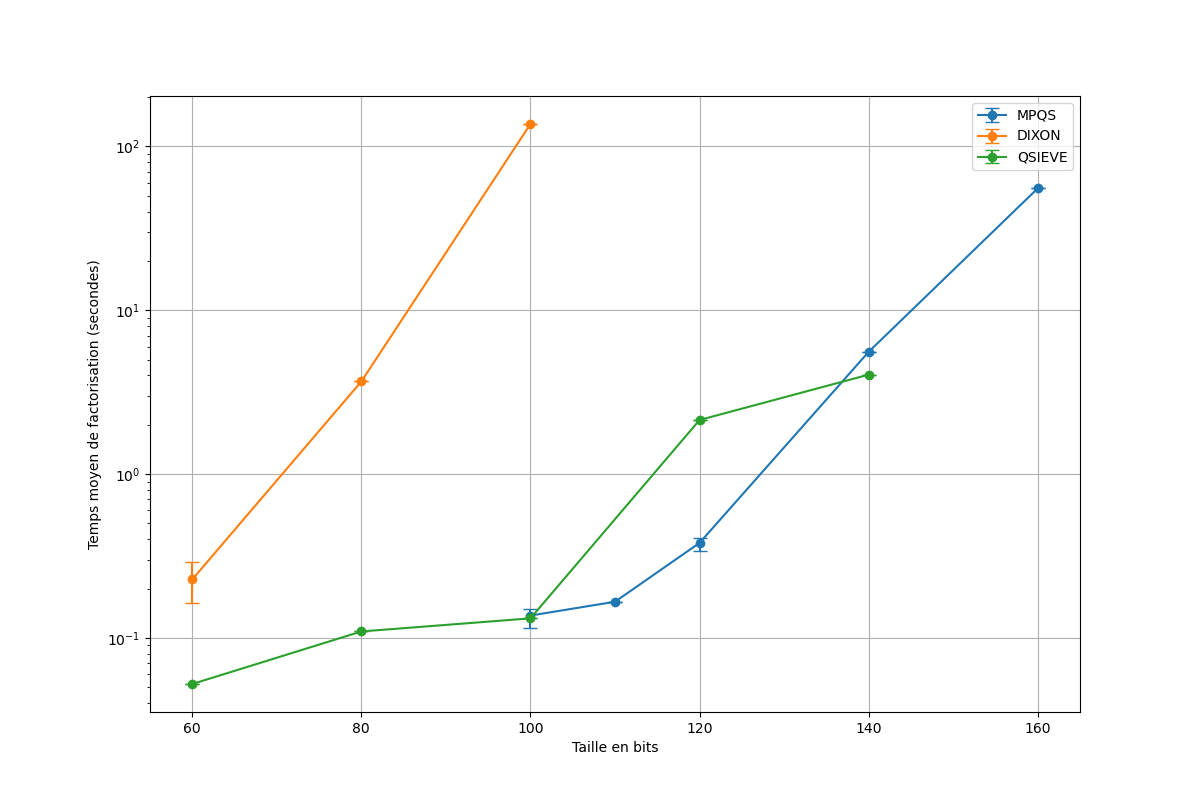
\includegraphics[width=13cm]{../tests/optimization_plot.png}}\par
    \endgroup
\end{frame}
}

\section{Annexe}
\addtocounter{framenumber}{-1}
\setbeamertemplate{footline}{}
\subsection*{Démonstrations}


\label{demo:congdecarre}
\begin{frame}
    \addtocounter{framenumber}{-1}
    \begin{block}{Proposition}
    Soient $b\in \mathbb N, (x_i)_{i\in \llbracket 1, b+1\rrbracket}\in \mathbb N^{b+1}$
    et $(v_i)_{i\in \llbracket 1, b+1\rrbracket}\in \mathbb F_2^b$ les vecteurs valuations de $x_i^2 \pmod N$ pour $i \in \llbracket 1,b+1 \rrbracket$
    et finalement $(\lambda_i)_{i \in \llbracket 1,b+1 \rrbracket}\in \mathbb \{0,1\}^{b+1}$ tels que,
    \[
    \sum_{i=1}^{b+1} \lambda_iv_i = 0_{\mathbb F_2^b} = (2\alpha_1, \dots, 2\alpha_b)
    \]
    \newline
    On pose $y = \prod_{j=1}^b p_j^{\alpha_j}$ et $x = \prod_{j=1}^{b+1}x_j^{\lambda_j}$, alors $x ^2 \equiv y ^2 \pmod N$
    \end{block}
\end{frame}

\begin{frame}
    \addtocounter{framenumber}{-1}
    \begin{block}{Démonstration}
        \begin{align*}
            x^2 = (\prod_{i=1}^{b+1} x_i^2)^{\lambda_i} &\equiv \prod_{i=1}^{b+1} \prod_{j=1}^b p_j^{\lambda_iv_i^{(j)}} \pmod N\\
            &\equiv \prod_{j=1}^b \prod_{i=1}^{b+1} p_j^{\lambda_iv_i^{(j)}} \pmod N\\
            &\equiv \prod_{j=1}^b p_j^{\sum_{i =1}^{b+1}\lambda_iv_i^{(j)}} \pmod N\\
            &\equiv (\prod_{j=1}^b p_j^{\alpha_j})^2 \pmod N \qquad\quad (\text{déf de } \alpha_j) \\ % cursed but works
            &\equiv y^2 \pmod N
        \end{align*}
    \end{block}
\end{frame}

\label{demo:qx}
\begin{frame}
    \addtocounter{framenumber}{-1}
    \begin{block}{Proposition}
        Si $Q = (\lfloor\sqrt N\rfloor + X)^2 - N$, alors $p\mid Q(x) \implies \forall k\in \mathbb N,  p\mid Q(x+kp)$
    \end{block}
    \begin{block}{Démonstration}
    En effet, supposons $p\mid Q(x)$, on a:
    \begin{align*}
        Q(x+kp) &= (\lfloor\sqrt N\rfloor + x+kp)^2 - N \\
                &= Q(x) + 2kp(\lfloor\sqrt N\rfloor+ x) + k^2p^2 \\
                &= Q(x) + p\times(2k(\lfloor\sqrt N\rfloor + x) + k^2p)
    \end{align*}
    d'où $p\mid Q(x+kp)$
    \end{block}
\end{frame}

{
\UseRawInputEncoding

%Make plain
\setbeamertemplate{headline}{}
\setbeamertemplate{navigation symbols}{}

% Import code command
\newcommand{\importcode}[1]{
    \begin{flushright}\textit{#1}\end{flushright}
    \begin{multicols}{2}
        \lstinputlisting[style=annexeStyle]{#1}
    \end{multicols}
    \pagebreak
}
%

\subsection*{Codes}

\importcode{../c/vector.h}
\importcode{../c/vector.c}
\importcode{../c/tonellishanks.h}
\importcode{../c/tonellishanks.c}
\importcode{../c/system.h}
\importcode{../c/system.c}
\importcode{../c/parse\_input.h}
\importcode{../c/parse\_input.c}
\importcode{../c/list\_matrix\_utils.h}
\importcode{../c/list\_matrix\_utils.c}
\importcode{../c/factorbase.h}
\importcode{../c/factorbase.c}
\importcode{../c/main.c}

\importcode{../c/dixon/dixon.h}
\importcode{../c/dixon/dixon.c}

\importcode{../c/qsieve/qsieve.h}
\importcode{../c/qsieve/qsieve.c}

\importcode{../c/mpqs/common\_mpqs.h}
\importcode{../c/mpqs/common\_mpqs.c}
\importcode{../c/mpqs/polynomial.h}
\importcode{../c/mpqs/polynomial.c}
\importcode{../c/mpqs/mpqs.h}
\importcode{../c/mpqs/mpqs.c}
\importcode{../c/mpqs/parallel\_mpqs.h}
\importcode{../c/mpqs/parallel\_mpqs.c}
}
\end{document}